{$\space$\par}
\vspace{0.5cm}
\justifying
\section*{{\bfseries \LARGE Questão 4 -} {\bfseries \large  Crie uma função no R que receba um vetor de dados qualquer e forneça como resultado ao usuário: na tela gráfica, uma figura de dois painéis, um ao lado do outro, nos quais o primeiro mostra um gráfico qq-plot para a amostra fornecida e uma linha qqline vermelha tracejada de uma população normal; e no segundo, um histograma do vetor fornecido, acompanhado por um “tapete" de valores individuais na abscissa (comando rug) e de três barras verticais, sendo a central em linha sólida vermelha indicando o valor da média amostral, e as duas linhas laterais tracejadas verdes indicando o erro da média amostral, isto é, $\mu\pm \epsilon\mu$. Lembre-se que o erro da média amostral costuma ser chamado de “erro padrão”. Ainda, adicione nesse último painel a curva da melhor gaussiana ajustada aos dados fornecidos.}}

\vspace{0.2cm}

\textcolor{red}{O plot de quantil-quantil é muito útil para uma análise exploratória da gaussianidade dos dados. Além dele, também podemos fazer uma investigação visual no histograma dos dados e comparar com um ajuste da melhor gaussiana. Para essa análise, utilizando o método de máxima verossimilhança, que seleciona os parâmetros que maximizam $\prod_{i=1}^nf(X_i;\theta)$ no ajuste.
Para demostrar a função, criei um vetor com a soma de 3 distribuições diferentes e os resultados se encontram na imagem.
}

\vspace{0.8cm}

\begin{figure}[h]
    \centering
    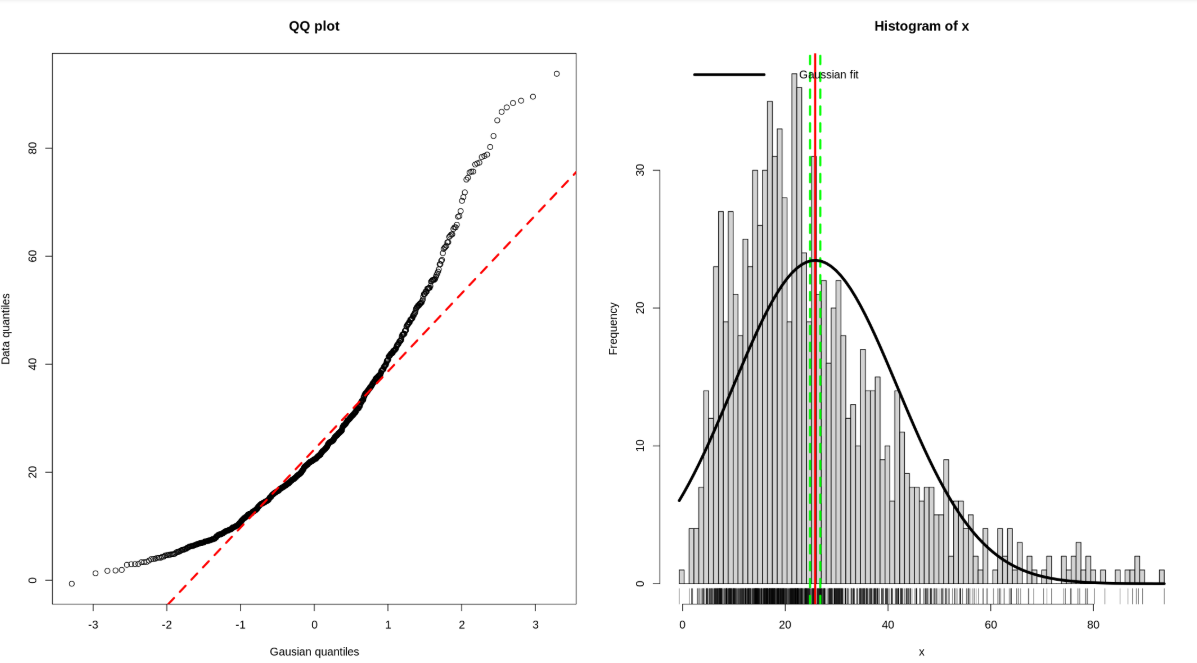
\includegraphics[width=0.9\linewidth]{Figuras/Captura de tela 2025-06-01 105629.png}
\end{figure}

\newpage

\begin{lstlisting}
    analysis = function(x){
        par(mfcol=c(1,2))
        options(repr.plot.width=18,repr.plot.height=10)
        
        # QQ plot
        qqnorm(x, xlab='Gausian quantiles', ylab = 'Data quantiles', main='QQ plot')
        qqline(x, col='red', lwd=3, lty=2)
        
        # Histogram
        hist(x, breaks=seq(min(x), max(x), length.out = 100))
        rug(x)
        
        # Estimating mean and its error
        results = t.test(x)
        abline(v=results$estimate, col='red', lwd=3)
        abline(v=results$conf.int[1], col='green', lty=2, lwd=3)
        abline(v=results$conf.int[2], col='green', lty=2, lwd=3)
        
        # Fitting a gaussian dist
        fit = fitdist(x, 'norm', 'mle')
        x_plot = seq(min(x), max(x), length.out = 100)
        weight = (max(x)-min(x))/100 * length(x)
        y_plot = dnorm(x_plot, mean=fit$estimate[1], sd=fit$estimate[2])*weight
        lines(x_plot, y_plot, lwd=4)
        legend('topleft', legend='Gaussian fit', lwd=4, col='black', box.lwd=0)
    }
    
    vetor = rpois(1000,lambda = 3)+rnorm(1000) + 6*rchisq(1000,df=4)
    analysis(vetor)
\end{lstlisting}

